
\documentclass[letterpaper,english,12pt]{article}
\usepackage{%
	amsfonts,%
	amsmath,%	
	amssymb,%
	amsthm,%
	babel,%
	bbm,%
	%biblatex,%
	caption,%
	centernot,%
	color,%
	enumerate,%
	%enumitem,%
	epsfig,%
	epstopdf,%
	etex,%
	fancybox,%
	framed,%
	fullpage,%
	%geometry,%
	graphicx,%
	hyperref,%
	latexsym,%
	mathptmx,%
	mathtools,%
	multicol,%
	pgf,%
	pgfplots,%
	pgfplotstable,%
	pgfpages,%
	proof,%
	psfrag,%
	%subfigure,%	
	tikz,%
	times,%
	ulem,%
	url,%
	xcolor,%
	mathpazo
}

\definecolor{shadecolor}{gray}{.95}%{rgb}{1,0,0}
\usepackage[margin=1in,top=0.75in]{geometry}
\usepackage[mathscr]{eucal}
\usepgflibrary{shapes}
\usepgfplotslibrary{fillbetween}
\usetikzlibrary{%
  arrows,%
  backgrounds,%
  chains,%
  decorations.pathmorphing,% /pgf/decoration/random steps | erste Graphik
  decorations.text,% 
  matrix,%
  positioning,% wg. " of "
  fit,%
  patterns,%
  petri,%
  plotmarks,%
  scopes,%
  shadows,%
  shapes.misc,% wg. rounded rectangle
  shapes.arrows,%
  shapes.callouts,%
  shapes%
}

%\pgfplotsset{compat=newest} %<------ Here
\pgfplotsset{compat=1.11} %<------ Or use this one

\theoremstyle{plain}
\newtheorem{thm}{Theorem}[section]
\newtheorem{lem}[thm]{Lemma}
\newtheorem{prop}[thm]{Proposition}
\newtheorem{cor}[thm]{Corollary}
\newtheorem{clm}[thm]{Claim}

\theoremstyle{definition}
\newtheorem{axiom}[thm]{Axiom}
\newtheorem{defn}[thm]{Definition}
\newtheorem{conj}[thm]{Conjecture}
\newtheorem{exmp}[thm]{Example}
\newtheorem{exerc}[thm]{Exercise}
\newtheorem{assum}[thm]{Assumptions}

\theoremstyle{remark}
\newtheorem{rem}[thm]{Remark}
\newtheorem{note}[thm]{Note}

\newcommand{\Cov}{\operatorname{Cov}}
%\newcommand{\det}{\operatorname{det}}
\newcommand{\Real}{\mathbb{R}}
\newcommand{\tr}{\operatorname{tr}}
%\newcommand{\Var}{\operatorname{Var}}

\DeclareMathOperator{\sign}{sign}
%\renewcommand{\proof}[1]{\begin{proof}#1\end{proof}}
\newcommand{\EQ}[1]{\begin{equation*}#1\end{equation*}}
\newcommand{\EQN}[1]{\begin{equation}#1\end{equation}}
\newcommand{\eq}[1]{\begin{align*}#1\end{align*}}
\newcommand{\meq}[2]{\begin{xalignat*}{#1}#2\end{xalignat*}}
\newcommand{\norm}[1]{\left\lVert#1\right\rVert}
\newcommand{\abs}[1]{\left\lvert#1\right\rvert}
\newcommand{\expect}[1]{\mathbb{E}\left[{#1}\right]}
\newcommand{\prob}[1]{\mathbb{P}\left[{#1}\right]}
\newcommand{\given}{\; \big\vert \;} 
\newcommand{\set}[1]{\left\{#1\right\}} 
\newcommand{\indicator}[1]{\mathbb{1}_{\set{#1}}} 
\newcommand{\inner}[1]{\left\langle#1\right\rangle}
\newcommand{\red}[1]{\textcolor{red}{#1}} 
\newcommand{\E}[1]{\mathbb{E}\left[#1\right]}
\newcommand{\Var}[1]{\operatorname{Var}\left[#1\right]}

\newcommand{\D}{\mathbb{D}}
%\newcommand{\E}{\mathbb{E}}
\newcommand{\N}{\mathbb{N}}
\renewcommand{\P}{\mathbb{P}}
\newcommand{\Q}{\mathbb{Q}}
\newcommand{\R}{\mathbb{R}}
\newcommand{\Z}{\mathbb{Z}}

\newcommand{\bU}{\mathbf{1}}
\newcommand{\bx}{\mathbf{x}}

\newcommand{\cB}{\mathcal{B}}
\newcommand{\cC}{\mathcal{C}}
\newcommand{\cD}{\mathcal{D}}
\newcommand{\cF}{\mathcal{F}}
\newcommand{\cG}{\mathcal{G}}
\newcommand{\cH}{\mathcal{H}}
\newcommand{\cO}{\mathcal{O}}
\newcommand{\cT}{\mathcal{T}}
\newcommand{\cX}{\mathcal{X}}
\newcommand{\cY}{\mathcal{Y}}

\newcommand{\sA}{\mathscr{A}}
\newcommand{\sB}{\mathscr{B}}
\newcommand{\sC}{\mathscr{C}}
\newcommand{\sD}{\mathscr{D}}
\newcommand{\sE}{\mathscr{E}}
\newcommand{\sF}{\mathscr{F}}
\newcommand{\sG}{\mathscr{G}}
\newcommand{\sH}{\mathscr{H}}
\newcommand{\sL}{\mathscr{L}}
\newcommand{\dO}{\mathscr{O}}
\newcommand{\sS}{\mathscr{S}}
\newcommand{\sT}{\mathscr{T}}
\newcommand{\sX}{\mathscr{X}}
\newcommand{\sY}{\mathscr{Y}}
\newcommand{\sZ}{\mathscr{Z}}

% Debug
\newcommand{\todo}[1]{\begin{color}{blue}{{\bf~[TODO:~#1]}}\end{color}}

% a few handy macros

\renewcommand{\le}{\leqslant}
\renewcommand{\ge}{\geqslant}
\newcommand\matlab{{\sc matlab}}
\newcommand{\goto}{\rightarrow}
\newcommand{\bigo}{{\mathcal O}}
%\newcommand{\half}{\frac{1}{2}}
%\newcommand\implies{\quad\Longrightarrow\quad}
\newcommand\reals{{{\rm l} \kern -.15em {\rm R} }}
\newcommand\complex{{\raisebox{.043ex}{\rule{0.07em}{1.56ex}} \hskip -.35em {\rm C}}}


% macros for matrices/vectors:

% matrix environment for vectors or matrices where elements are centered
\newenvironment{mat}{\left[\begin{array}{ccccccccccccccc}}{\end{array}\right]}
\newcommand\bcm{\begin{mat}}
\newcommand\ecm{\end{mat}}

% matrix environment for vectors or matrices where elements are right justifvied
\newenvironment{rmat}{\left[\begin{array}{rrrrrrrrrrrrr}}{\end{array}\right]}
\newcommand\brm{\begin{rmat}}
\newcommand\erm{\end{rmat}}

% for left brace and a set of choices
%\newenvironment{choices}{\left\{ \begin{array}{ll}}{\end{array}\right.}
\newcommand\when{&\text{if~}}
\newcommand\otherwise{&\text{otherwise}}
% sample usage:
%  \delta_{ij} = \begin{choices} 1 \when i=j, \\ 0 \otherwise \end{choices}


% for labeling and referencing equations:
\newcommand{\eql}{\begin{equation}\label}
\newcommand{\eqn}[1]{(\ref{#1})}
% can then do
%  \eql{eqnlabel}
%  ...
%  \end{equation}
% and refer to it as equation \eqn{eqnlabel}.  


% some useful macros for finite difference methods:
\newcommand\unp{U^{n+1}}
\newcommand\unm{U^{n-1}}

% for chemical reactions:
\newcommand{\react}[1]{\stackrel{K_{#1}}{\rightarrow}}
\newcommand{\reactb}[2]{\stackrel{K_{#1}}{~\stackrel{\rightleftharpoons}
   {\scriptstyle K_{#2}}}~}


\makeatletter
\def\th@plain{%
  \thm@notefont{}% same as heading font
  \itshape % body font
}
\def\th@definition{%
  \thm@notefont{}% same as heading font
  \normalfont % body font
}
\makeatother
\date{}

\graphicspath{{./Figures/}}
%\usepackage{witharrows}
%opening
\title{Lecture-10: Many Random Variables}
\author{Vivek VP}

\begin{document}
\maketitle
\section{Qualitative view of Random Variables}
Physical systems of particles can be modelled by assigning a random variable to state of each particles. Here we assume the particles have no interaction or interaction is minimal. Thus for $N$ particles we have an $N$ length vector $\underbar x = (x_1,x_2,\dots ,x_N)$ with probability 
\begin{equation}
  P_N(\underbar x) = P_N(X_1,\dots ,x_N) .
\end{equation}
An instance of this would be Boltzmann distribution for a physical system with $N$ degrees of freedom. Shannon Entropy of this distribution is 
  \begin{equation}
      H_N = -\E {log P_N(\underbar x) }
  \end{equation}
  Typically $H_N$ grows linearly with $N$ for large $N$. So entropy per variable $h_n=H_N/N$ has a finite limit;so we define a quantity $h$.
  
 \begin{defn}
 	$h: \lim_{N\to\infty} h_N$
 \end{defn}
  We will be interested in defining the quantity 
  \begin{equation}
      r(\underbar x) = 1/N log \big[ 1/P_N(\underbar x)\big]
  \end{equation}
  to characterize any particular realization $\underbar{x}$. We would like to know how close is $r(x)$ to $h_N$. In most cases $r(x)$ is peaked around $r=h_N$. Often probability distribution of $r(\underbar x)$ behave exponentially with 
  \begin{equation}
   P\lbrace r(x) \approx \rho \rbrace=e^{-NI(\rho)}
   \end{equation}
   where
   $I(\rho)$ has minimum at $\rho = h$.
   and $I(h)=0$
   From this observation and (3) we have 
   \begin{equation}
       P_N(x) = e^{-Nh}
   \end{equation}
   Total probability of realization $\underbar x$ with $r(x) \approx h$ is 1. This will imply that number of configurations with major contribution to probability is $e^{Nh}. $This in general is a  small number when compared to total number of configurations $\sX^N$. 
   \begin{equation}
   	\text{Number of typical configurations}=e^{Nh}<<\sX^N
   \end{equation}
   This has a lot of implications.For example if we want to estimate an observable $\mathcal{O}$ we can sample configuration and it will give good estimates because major part of total probability is distributed among typical configurations. But it takes orderof $e^{N(\log\abs{\mathcal{X}})-h}$ time to generate a sample. Monte Carlo methods provide better solution for this problem
  \section{Large deviations for independent variables}
  \begin{thm}(Sanov) Let $s1,\dots s_N\in\mathcal{X}$ be $N$ i.i.d random variables drawn from the probability distribution $p(x)$, and let $K\subset \mathcal{M(X)}$ be a compact set of probability distributions over $\mathcal{X}$. If $q$ is the type of $(s1,\dots,s_N)$ then
  \begin{equation}
      \P\big[q\in K\big]= e^{-ND(q^*\parallel p)}
  \end{equation}
  where $q^* = \text{arg min}_{q\in K}D(q\parallel p)$, and $D(q\parallel p)$ is the Kullback-Leibler divergence.
  \end{thm}
  
% \begin{aligned}
%   \mathds{P}\big[q\in K] &= \sum_{q'\in K}P[q_s=q']\\ 
 
%   \end{aligned}

\begin{proof} 
  Now for a particular $q'$ 
  \begin{equation} \label{sanov1}
  \begin{split}
      (P(q_{s}=q')) & =  \prod_{x\in \mathcal{X}}^{} P(Nq'(x) \text{times $x$ appears in s)}\\
      & ={N \choose Nq'(x_1), Nq'(x_2), \dots, Nq'(x_{\abs{\mathcal{X}}})} \prod_{x \in \mathcal{X}} p(x)^{Nq'(x)}\\
      & ={N! \choose{Nq'(x_1)}!,Nq'(x_2)!,\dots,Nq'(x_{\abs{\mathcal{X}}})!} \prod_{x \in \mathcal{X}} p(x)^{Nq'(x)}\\
    %   & ={N \choose{Nq'(x_1)},Nq'(x_2),\dots,Nq'(x_{\abs(\mathcal{X}))}}
  \end{split}
  \end{equation}
  
  Using Stirlings equation 
  \begin{equation}
  \log_2 n! = n \log_2 n
  \end{equation}
  
  \begin{equation}
    n! = 2^{n\log_2 n} \label{sanov2}
  \end{equation}
  
  
  \begin{equation} \label{sanov3}
  \dfrac{N!}{(Nq'(x_1))! (Nq'(x_2))! \dots (Nq'(x_{\abs{\mathcal{X}}}))!} 
  =  2^{N\log N - Nq_1\log{Nq_1} - Nq_2\log{Nq_2} \dots Nq_{\abs{\mathcal{X}}} \log{Nq_{\abs{\mathcal{X}}}}}
  \end{equation}
  
  \begin{equation} \label{sanov4}
      \prod_{x \in \mathcal{X}} p(x)^{Nq'(x)}= \prod_{x \in \mathcal{X}} 2^{Nq'(x)\log p(x)}
  \end{equation}
  We have KL Divergence D as 
  \begin{equation}
      D(q \Vert p) = \sum_{x}{}q(x)\log \dfrac{q(x)}{p(x)}
  \end{equation}
  From $\ref{sanov1},~\ref{sanov2},~\ref{sanov3},~\ref{sanov4}$ we have
  \begin{equation}
      P(q_{s}=q') = \prod_{x\in \mathcal{X}}2^{-ND(q \Vert p)}
  \end{equation}
  By approximating with leading term in exponential
  we have 
  \begin{equation}
       P(q_{s}=q') = e^{-ND(q* \Vert p)}
  \end{equation}
  \end{proof}
  
 \begin{exmp}
 
 A simple model of a column of the atmosphere is obtained by considering $N$ particles in the earth's gravitational field.The state of particle $i \in \lbrace 1,2, \dots, N \rbrace $ is given by a single coordinate $z_i\geq 0$ which measures its height with respect to level. To simplify , we make assumption $z_i$ is integer.
 \begin{equation}
     E=\sum_{i=1}{N}z_i
 \end{equation}
 Consider a configuration $:{z_1,\dots,z_N}$. Its type can be interpreted as:
 \begin{equation}
   \rho(z) = \displaystyle 1/N\sum_{i=1}^{N}\indicator{z=z_i}  
 \end{equation}
 
 \begin{equation}
     \rho_{eq}(z)=\langle \rho(z) \rangle = (1-e^{-\beta})e^{-\beta z}
 \end{equation}
 Using Boltzmann probability distribution; expected density profile can be computed as follows.
 \begin{equation}
 \text{Partition function   } \label{pf}
	Z(\beta)= \sum_{x \in \sX}^{} e^{-E(x)}
 	=\sum_{z=0}^{\infty} e^{-\beta z} = \frac{1}{1-e^{-\beta}}. 
 \end{equation}
 So probability distribution follows
 
 \begin{equation}
 	\mu_{\beta}(x) = \frac{1}{Z(\beta)}e^{-\beta E(x)} = (1-e^{-\beta})e^{-\beta z}
 \end{equation}
 
 We compute the probability of getting a general exponential density profile with parameter $\lambda$:
 \begin{equation}
 	\rho_{\lambda}(z)= (1-e^{-\lambda})e^{-\lambda z}
 \end{equation}
 For that we find the KL divergence between $\rho_{\lambda}$ and $\rho_{eq}$
 \begin{equation}
     D(\rho_{\lambda} \Vert \rho_{eq}) = 
     \sum_{z}^{} \rho_{\lambda}(z) \log \frac{\rho_{\lambda}(z)}{\rho_{eq}(z)} =     
     \log{  \frac{1-e^{-\lambda}}{1-e^{-\beta}}  + \frac{\beta -\lambda}{e^{\lambda}-1}}
 \end{equation}
 We now plot KL divergence as a function of $\lambda$ in figure \ref{fig:Earthatmo}.
 \begin{equation}
 	I_{\beta}(\lambda)= D(\rho_{\lambda} \Vert \rho_{eq})
 \end{equation}
 \begin{figure}[h!] \label{fig}
  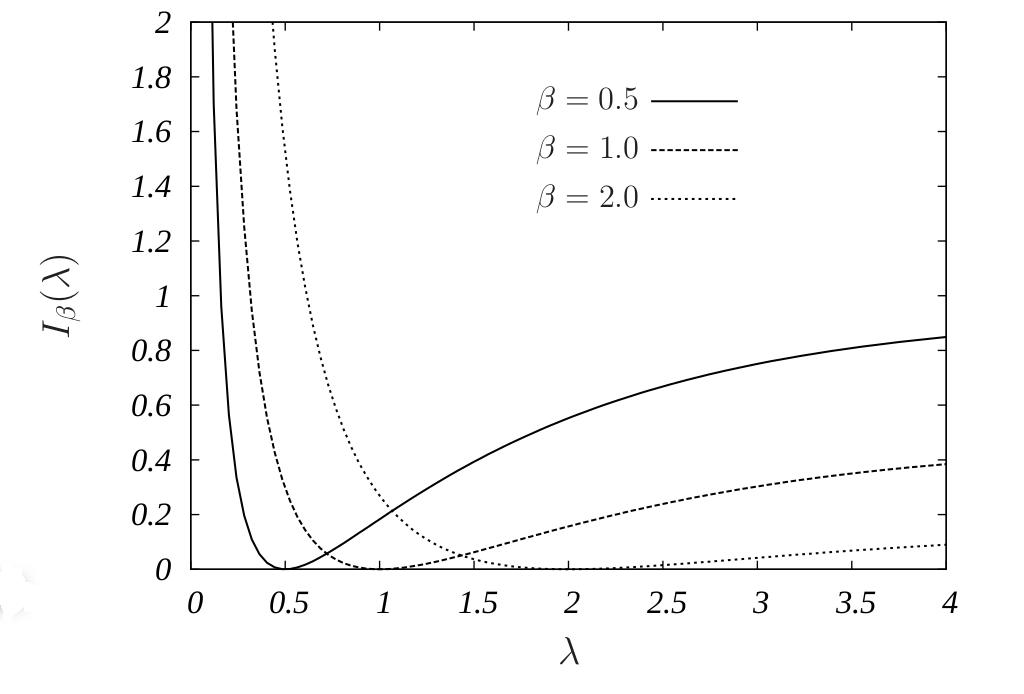
\includegraphics[width=\linewidth]{EarthAtmo.jpeg}
  \caption{Equilbrium density profile}
  \label{fig:Earthatmo}
\end{figure}
It can be noted from the figure \ref{fig:Earthatmo} that small values of $\lambda$ are very rare.
 \end{exmp}
 \section{How typical is an empirical average?}
%  $\bar{f}$
 The empirical average of a measurement is given by:
 \begin{equation}
     \bar{f} = \frac{1}{N}\sum_{i=1}^{N}f(s_i)
 \end{equation}
 \begin{cor}
 Let $s1,\dots ,s_N$ be $N$ i.i.d random variables drawn from a probability distribution $p(.)$. Let $f:\mathcal{X}\rightarrow \R$ be a real-valued  function and let $\bar{f}$ be its empirical average. If $A\subset R$ is a closed interval of the real axis, then 
 \begin{equation}
     \P\big[\bar{f}\in A]= e^{[-NI(A)]},
 \end{equation}
 where
 \begin{equation}
     I(A)=\min_q\big[D(q\Vert p)| \sum_{x\in \sX}^{} q(x)f(x) \in A]
 \end{equation}
 \end{cor}
 \begin{proof}
 We note that $\bar{f}$ is related to the type of sequence $x_1,x_2,\dots x_n$ as $\bar{f}=\sum_{x}^{}q(x)f(x)$. Keeping in mind Sanov theorem , we define a set as follows 
 \begin{equation}
     K= \Big\{ q\in \mathcal{M}(\sX)|\sum_{x\in \sX}^{} q(x)f(x) \in A \Big\}
 \end{equation}
 Then the result follows directly from Sanov by camparing K with set in Sanov and $I(A)$ with $D(q^* \Vert p)$.
 \end{proof}
 
 \begin{exmp}
 	Let $s_1,...,s_N$ be $N$ i.i.d random variablesdrawn from a probability distribution $p(.)$ with bounded support. Show that, to leading exponential order, 
   \begin{equation}
       \P \{s_1 + \dots + s_N \leq  = 0\} = \{ \inf_{z\geq 0} \E {e^{-zs_1}}  \}^N
   \end{equation}
     
 \end{exmp}
 
 \begin{exmp}
   We look at N particles in a gravitational field, and consider the average height of the particles 
   \begin{equation}
       \bar{z}= \dfrac{1}{N}\sum_{i=1}^{N}z_i.
    \end{equation}
     Expected value of this quantity  is 
       \begin{equation}
           \E{\bar{z}}= z_{eq}= (e^\beta -1)^{-1}.
           \end{equation}
           The probability of a fluctuation in $\bar{z}$ is easily computed using the obove corollary.For $z>z_{eq}$ we obtain 
           \begin{equation}
               \P(z>\bar{z}) = e^{-NI(z)},
           \end{equation}
           where 
           \begin{equation}
               I(z) = \big(1+z\big)\log \big( \dfrac{1+z_{eq}}{1+z}\big) + z\log{\big(\dfrac{z}{z_{eq}}\big)}
           \end{equation}
           
       
   
 \end{exmp}


\end{document}